\providecommand{\Mod}{\mathbb{M}od}
\providecommand{\Fun}{\operatorname{Fun}}
\providecommand{\rvnullpair}{\vcenter{\hbox{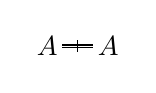
\begin{tikzpicture}[x=1em,y=1em]%
\node (rva) at (0,0) {$A$};\node (rvb) at (2.2,0) {$A$};%
\draw[double] (0.55,0) -- (1.65,0);\draw (1.1,0.22) -- (1.1,-0.22);\end{tikzpicture}}}}

\section{双侧等价纤维化的\trDoubleCategory}\label{sec:double-category-of-two-sided-isofibrations}

回忆推论 7.4.4：\trModule{}的\trInfinityCosmos{}既可定义为%
\trTwoSidedFibration{}的\trInfinityCosmos{}的一个全子范畴，也可定义为%
\trTwoSidedIsofibration{}的\trInfinityCosmos{}的一个全子范畴。
这为构造模的\trVirtualDoubleCategory{}摆出了两条路线：它既可以实现为双侧纤维化的\trDoubleCategory{}的
一个全子范畴，也可以实现为双侧等价纤维化的\trDoubleCategory{}的一个全子范畴。我们采纳
后者，因为它略为简单；不过也邀请读者改走前一条路线（见%
\cref{ex:map-of-two-sided-fibrations}）。

我们的第一项任务，是定义将要引入的那些\trDoubleCategory{}中的 2 维态射。

\begin{definition}\label{def:fibered-map-of-two-sided-isofibrations}
从 $A\overset{q}{\twoheadleftarrow}E\overset{p}{\twoheadrightarrow}B$ 到
$A\overset{s}{\twoheadleftarrow}F\overset{r}{\twoheadrightarrow}B$ 的一支%
\textbf{双侧等价纤维化间的纤维化映射}（fibered map of two-sided
isofibrations），是一个由严格交换的\trFunctor{}构成的纤维化同构类
\begin{center}
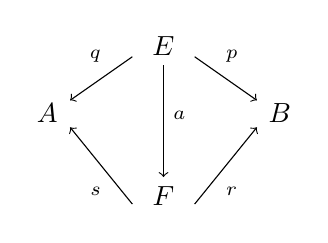
\begin{tikzpicture}[x=1.5em,y=1.5em]
  \node (E) at (0,1.6)  {$E$};
  \node (A) at (-2.8,0) {$A$};
  \node (B) at (2.8,0)  {$B$};
  \node (F) at (0,-2.0) {$F$};
  \draw[->] (-0.75,1.35) -- node[above left,pos=0.35]{$\scriptstyle q$} (-2.25,0.3);
  \draw[->] (0.75,1.35)  -- node[above right,pos=0.35]{$\scriptstyle p$} (2.25,0.3);
  \draw[->] (0,1.15) -- node[right,pos=0.45]{$\scriptstyle a$} (0,-1.55);
  \draw[->] (-0.75,-2.2) -- node[below left,pos=0.35]{$\scriptstyle s$} (-2.25,-0.35);
  \draw[->] (0.75,-2.2)  -- node[below right,pos=0.35]{$\scriptstyle r$} (2.25,-0.35);
\end{tikzpicture}
\end{center}
其中两支这样的\trFunctor{} $a$ 与 $a'$ 被视为等价的，当存在自然同构
$\gamma\colon a\cong a'$ 使得 $s\gamma=\mathrm{id}_{q}$ 且
$r\gamma=\mathrm{id}_{p}$。

当 $A\overset{q}{\twoheadleftarrow}E\overset{p}{\twoheadrightarrow}B$ 与
$A\overset{s}{\twoheadleftarrow}F\overset{r}{\twoheadrightarrow}B$ 是%
\trModule{}时，我们把二者之间的纤维化映射称作从 $E$ 到 $F$ 的%
\textbf{模的纤维化映射}（fibered map of modules）。
\end{definition}

\begin{observation}[模与纤维化映射的 1-范畴]\label{obs:one-categories-of-modules}
∞-宇宙 $\mathcal{K}$ 中从 $A$ 到 $B$ 的双侧等价纤维化连同纤维化映射一起
构成的 1-范畴可以这样得到：取以\trQuasiCategory{}富集的范畴
$\mathcal{K}_{/A\times B}$ 的一个商，或取其\trHomotopyTwoCategory{}
$\mathfrak{h}(\mathcal{K}_{/A\times B})$ 的一个商，或取切片%
\trHomotopyTwoCategory{} $\mathfrak{h}\mathcal{K}_{/A\times B}$ 的一个商。
这个商 1-范畴拥有同一批对象，并以诸\trFunctor{}的\trIsomorphism{}类作为
其态射。

由引理 7.4.3，从 $A$ 到 $B$ 的\trModule{}连同纤维化映射一起构成的 1-范畴
是一个全子范畴；或者换个说法，可以同法把它视为以\trKanComplex{}富集的
范畴 ${}_{A\backslash}\Mod(\mathcal{K})_{/B}$ 的商，或其%
\trHomotopyTwoCategory{} $\mathfrak{h}({}_{A\backslash}\Mod(\mathcal{K})_{/B})$
的商。
\end{observation}

\cref{obs:one-categories-of-modules}的诸 1-范畴之所以有趣，是因为它们恰好
捕捉了定义 3.2.7 中首次引入的、双侧等价纤维化之间或模之间的那个正确的%
\trEquivalence{}概念。

\begin{lemma}\label{lem:one-category-equivalences}
在∞-宇宙 $\mathcal{K}$ 中：
\begin{enumerate}[label=(\roman*)]
\item 一对双侧等价纤维化在 $\mathcal{K}_{/A\times B}$ 中\trEquivalence{}，
当且仅当它们在从 $A$ 到 $B$ 的双侧等价纤维化的 1-范畴中\trIsomorphism{}；
\item 一对\trModule{}在 $A\times B$ 之上\trEquivalence{}，当且仅当它们在从
$A$ 到 $B$ 的模的 1-范畴中\trIsomorphism{}。
\end{enumerate}
\end{lemma}

刚才呈现的每一个定义都容有一个共同的推广，它定义了居于方块之中的那些
2 维映射。

\begin{definition}[方块中的映射]\label{def:maps-in-squares}
从 $A'\overset{q'}{\twoheadleftarrow}E'\overset{p'}{\twoheadrightarrow}B'$
到 $A\overset{q}{\twoheadleftarrow}E\overset{p}{\twoheadrightarrow}B$ 的、
位于 $f\colon A'\to A$ 与 $g\colon B'\to B$ 之上的一个\textbf{模映射}
（map of modules）或\textbf{双侧等价纤维化映射}（map of two-sided
isofibrations）描绘如下
\begin{center}
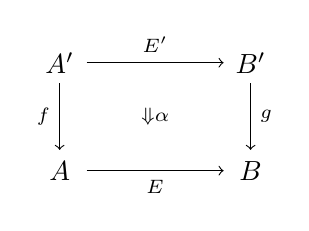
\begin{tikzpicture}[x=1.5em,y=1.5em]
  \node (Ap) at (0,1.3)    {$A'$};
  \node (Bp) at (4.6,1.3)  {$B'$};
  \node (A)  at (0,-1.3)   {$A$};
  \node (B)  at (4.6,-1.3) {$B$};
  \draw[->] (0.65,1.3) -- node[above]{$\scriptstyle E'$} (3.95,1.3);
  \draw[->] (0.65,-1.3) -- node[below]{$\scriptstyle E$} (3.95,-1.3);
  \draw[->] (0,0.8) -- node[left]{$\scriptstyle f$} (0,-0.8);
  \draw[->] (4.6,0.8) -- node[right]{$\scriptstyle g$} (4.6,-0.8);
  \node at (2.3,0) {$\scriptstyle\Downarrow\alpha$};
\end{tikzpicture}
\end{center}
它是一个由严格交换的\trFunctor{} $a$ 构成的纤维化同构类
\begin{center}
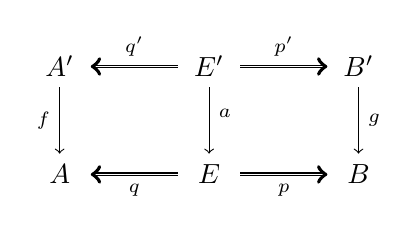
\begin{tikzpicture}[x=1.5em,y=1.5em]
  \node (Ap) at (0,1.3)    {$A'$};
  \node (Ep) at (3.6,1.3)  {$E'$};
  \node (Bp) at (7.2,1.3)  {$B'$};
  \node (A)  at (0,-1.3)   {$A$};
  \node (E)  at (3.6,-1.3) {$E$};
  \node (B)  at (7.2,-1.3) {$B$};
  \draw[double,->] (2.85,1.3) -- node[above]{$\scriptstyle q'$} (0.75,1.3);
  \draw[double,->] (4.35,1.3) -- node[above]{$\scriptstyle p'$} (6.45,1.3);
  \draw[double,->] (2.85,-1.3) -- node[below]{$\scriptstyle q$} (0.75,-1.3);
  \draw[double,->] (4.35,-1.3) -- node[below]{$\scriptstyle p$} (6.45,-1.3);
  \draw[->] (0,0.8) -- node[left]{$\scriptstyle f$} (0,-0.8);
  \draw[->] (3.6,0.8) -- node[right,pos=0.4]{$\scriptstyle a$} (3.6,-0.8);
  \draw[->] (7.2,0.8) -- node[right]{$\scriptstyle g$} (7.2,-0.8);
\end{tikzpicture}
\end{center}
其中两支这样的\trFunctor{} $a$ 与 $a'$ 被视为等价的，当存在自然同构
$\gamma\colon a\cong a'$ 使得 $q\gamma=\mathrm{id}_{aq'}$ 且
$p\gamma=\mathrm{id}_{bp'}$。
\end{definition}

\begin{observation}\label{obs:functor-space-over-product}
在\trModule{}或双侧等价纤维化的情形，从 $E'$ 到 $E$ 的、位于 $f\times g$
之上的映射所构成的\trFunctorSpace{} $\Fun_{f\times g}(E',E)$ 由如下\trPullback%
定义
\begin{center}
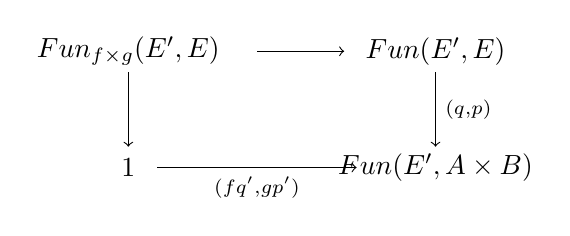
\begin{tikzpicture}[x=1.5em,y=1.5em]
  \node (Fl)  at (0,1.4)    {$\Fun_{f\times g}(E',E)$};
  \node (Ft)  at (7.4,1.4)  {$\Fun(E',E)$};
  \node (one) at (0,-1.4)   {$1$};
  \node (Fb)  at (7.4,-1.4) {$\Fun(E',A\times B)$};
  \draw[->] (3.1,1.4) -- (5.2,1.4);
  \draw[->] (7.4,0.9) -- node[right]{$\scriptstyle(q,p)$} (7.4,-0.9);
  \draw[->] (0,0.9) -- (0,-0.9);
  \draw[->] (0.7,-1.4) -- node[below]{$\scriptstyle(fq',gp')$} (5.5,-1.4);
  \node at (0.6,0.72) {$\scriptstyle\lrcorner$};
\end{tikzpicture}
\end{center}
正如在\cref{obs:one-categories-of-modules}中那样，模映射定义为该%
\trFunctorSpace{}中对象的\trIsomorphism{}类。
\end{observation}

现在我们引入双侧等价纤维化的\trDoubleCategory{}。这一结构既可以视为呈现于一个∞-宇宙
的\trHomotopyTwoCategory{} $\mathfrak{h}\mathcal{K}$ 中的诸数据之汇集，也
可以视为\cref{ex:cosmos-of-two-sided-isofibrations}所描述的那些以%
\trQuasiCategory{}富集的结构的商。
在某种意义上，后一观点更为自然，因为其水平复合由一个严格的\trUniversalProperty%
刻画，且不要求任何映射的同构类；但 2-范畴式的进路更为人熟悉，并且为发展%
\trInfinityCategories{}的形式范畴论提供了一个便利的舞台。

\begin{proposition}[双侧等价纤维化的\trDoubleCategory]%
\label{prop:double-category-of-two-sided-isofibrations}
一个∞-宇宙 $\mathcal{K}$ 的\trHomotopyTwoCategory{}承载一个（非幺的）%
\textbf{双侧等价纤维化的\trDoubleCategory}（double category of two-sided
isofibrations），其中：
\begin{itemize}
\item \textbf{对象}为\trInfinityCategories{}；
\item \textbf{竖直箭头}为\trFunctor{}；
\item \textbf{水平箭头} $A\xrightarrow{E}B$ 是双侧等价纤维化
$A\overset{q}{\twoheadleftarrow}E\overset{p}{\twoheadrightarrow}B$；并且
\item 以如下方块为边界的\textbf{\trCell}
\begin{center}
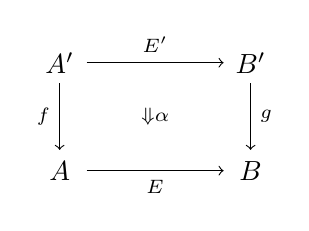
\begin{tikzpicture}[x=1.5em,y=1.5em]
  \node (Ap) at (0,1.3)    {$A'$};
  \node (Bp) at (4.6,1.3)  {$B'$};
  \node (A)  at (0,-1.3)   {$A$};
  \node (B)  at (4.6,-1.3) {$B$};
  \draw[->] (0.65,1.3) -- node[above]{$\scriptstyle E'$} (3.95,1.3);
  \draw[->] (0.65,-1.3) -- node[below]{$\scriptstyle E$} (3.95,-1.3);
  \draw[->] (0,0.8) -- node[left]{$\scriptstyle f$} (0,-0.8);
  \draw[->] (4.6,0.8) -- node[right]{$\scriptstyle g$} (4.6,-0.8);
  \node at (2.3,0) {$\scriptstyle\Downarrow\alpha$};
\end{tikzpicture}
\end{center}
是位于 $f\times g$ 上的双侧等价纤维化之间的映射；等价地，是\trQuasiCategory%
$\Fun_{f\times g}(E',E)$ 中对象的\trIsomorphism{}类。
\end{itemize}
\end{proposition}

\begin{proof}
箭头与胞腔的竖直复合即 $\mathcal{K}$ 中的复合。水平箭头的复合由命题 7.2.6
定义，而胞腔的水平复合由练习 7.2.i 定义。
由 $\mathcal{K}$ 中\trPullback{}与复合的\trSimplicial{}函子性，这两个构造
在典范自然同构的意义下都是结合的。
\end{proof}

刚才引入的这个\trDoubleCategory{}并不包含水平的单位箭头。出于技术上的原因，我们发现
把它们略去最为便利。

\begin{remark}[水平单位为何缺席]\label{rem:missing-horizontal-unit}
命题 7.2.6 所定义的跨度复合运算的单位是恒同跨度，而后者通常不是一条%
\trTwoSidedIsofibration{}。
与其把水平单位形式地添加到\cref{prop:double-category-of-two-sided-isofibrations}
的「\trDoubleCategory」之上，我们发现将它们略去更少引起混淆：因为当我们限制到最令我们
感兴趣的结构——模的\trVirtualEquipment——之上时，我们将看到，%
\trArrowInfinityCategory{}扮演着复合的水平单位这一角色，其意义将在命题
8.2.4 中得到描述，尽管对于跨度复合运算而言它并不定义一个水平复合单位。
\end{remark}

由练习 7.4.ii，\trModule{}在跨度复合之下并不构成\trDoubleCategory{}，这促使我们去寻找
另一种范畴结构来公理化它们的行为。
\trVirtualDoubleCategory{}是\trDoubleCategory{}的一种多范畴式类似物，适用于水平复合与单位可有可无的
场合。这一概念曾被 Burroni $[24]$ 与 Leinster $[76]$ 以各种名称研究过；
我们采用的是 Cruttwell 与 Shulman $[32]$ 的术语与记号。

\begin{definition}[\trVirtualDoubleCategory]\label{def:virtual-double-category}
一个\textbf{\trVirtualDoubleCategory}（virtual double category）由下列诸项构成：
\begin{itemize}
\item 一个由\textbf{对象}与\textbf{竖直箭头}构成的\trCategory{}；
\item 对任意一对对象 $A$、$B$，一个由\textbf{水平箭头} $A\to B$ 组成的
汇集；
\item 诸\textbf{\trCell}，其边界描绘如下
\begin{rveq}\label{eq:virtual-cell-boundary}
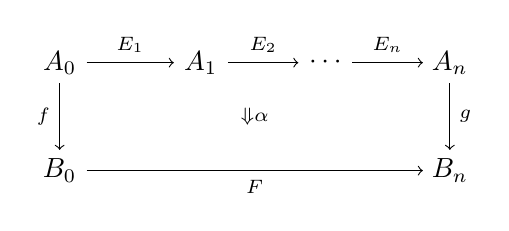
\begin{tikzpicture}[x=1.5em,y=1.5em]
  \node (A0) at (0,1.3)    {$A_{0}$};
  \node (A1) at (3.4,1.3)  {$A_{1}$};
  \node (Ad) at (6.4,1.3)  {$\cdots$};
  \node (An) at (9.4,1.3)  {$A_{n}$};
  \node (B0) at (0,-1.3)   {$B_{0}$};
  \node (Bn) at (9.4,-1.3) {$B_{n}$};
  \draw[->] (0.65,1.3) -- node[above]{$\scriptstyle E_{1}$} (2.75,1.3);
  \draw[->] (4.05,1.3) -- node[above]{$\scriptstyle E_{2}$} (5.75,1.3);
  \draw[->] (7.05,1.3) -- node[above]{$\scriptstyle E_{n}$} (8.75,1.3);
  \draw[->] (0,0.8) -- node[left]{$\scriptstyle f$} (0,-0.8);
  \draw[->] (9.4,0.8) -- node[right]{$\scriptstyle g$} (9.4,-0.8);
  \node at (4.7,0) {$\scriptstyle\Downarrow\alpha$};
  \draw[->] (0.65,-1.3) -- node[below]{$\scriptstyle F$} (8.75,-1.3);
\end{tikzpicture}
\end{rveq}
——包括在 $A_{0}=A_{n}$ 的情形下那些水平源长度为零的胞腔；
\item 对任何如下左图所示的构型，一个如下右图所示的\textbf{复合胞腔}
（composite cell）
\begin{rveq}\label{eq:virtual-composite-cell}
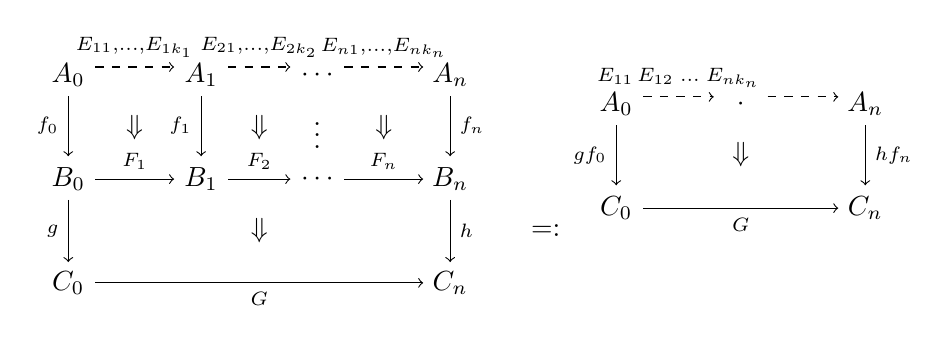
\begin{tikzpicture}[x=1.5em,y=1.5em]
  \node (A0) at (0,3.1)   {$A_{0}$};
  \node (A1) at (3.2,3.1) {$A_{1}$};
  \node (Ad) at (6.0,3.1) {$\cdots$};
  \node (An) at (9.2,3.1) {$A_{n}$};
  \draw[->,dashed] (0.65,3.3) -- node[above]{$\scriptstyle E_{11},\ldots,E_{1k_{1}}$} (2.55,3.3);
  \draw[->,dashed] (3.85,3.3) -- node[above]{$\scriptstyle E_{21},\ldots,E_{2k_{2}}$} (5.35,3.3);
  \draw[->,dashed] (6.65,3.3) -- node[above]{$\scriptstyle E_{n1},\ldots,E_{nk_{n}}$} (8.55,3.3);
  \draw[->] (0,2.6) -- node[left]{$\scriptstyle f_{0}$} (0,1.15);
  \draw[->] (3.2,2.6) -- node[left]{$\scriptstyle f_{1}$} (3.2,1.15);
  \node at (6.0,1.85) {$\vdots$};
  \draw[->] (9.2,2.6) -- node[right]{$\scriptstyle f_{n}$} (9.2,1.15);
  \node at (1.6,1.85) {$\Downarrow$};
  \node at (4.6,1.85) {$\Downarrow$};
  \node at (7.6,1.85) {$\Downarrow$};
  \node (B0) at (0,0.6)   {$B_{0}$};
  \node (B1) at (3.2,0.6) {$B_{1}$};
  \node (Bd) at (6.0,0.6) {$\cdots$};
  \node (Bn) at (9.2,0.6) {$B_{n}$};
  \draw[->] (0.65,0.6) -- node[above]{$\scriptstyle F_{1}$} (2.55,0.6);
  \draw[->] (3.85,0.6) -- node[above]{$\scriptstyle F_{2}$} (5.35,0.6);
  \draw[->] (6.65,0.6) -- node[above]{$\scriptstyle F_{n}$} (8.55,0.6);
  \draw[->] (0,0.1) -- node[left]{$\scriptstyle g$} (0,-1.4);
  \draw[->] (9.2,0.1) -- node[right]{$\scriptstyle h$} (9.2,-1.4);
  \node at (4.6,-0.65) {$\Downarrow$};
  \node (C0) at (0,-1.9)  {$C_{0}$};
  \node (Cn) at (9.2,-1.9){$C_{n}$};
  \draw[->] (0.65,-1.9) -- node[below]{$\scriptstyle G$} (8.55,-1.9);
  \node at (11.5,-0.65) {$=:$};
  \begin{scope}[shift={(13.2,0)}]
  \node (a0) at (0,2.4)   {$A_{0}$};
  \node (ad) at (3.0,2.4) {$\cdot$};
  \node (an) at (6.0,2.4) {$A_{n}$};
  \draw[->,dashed] (0.65,2.58) --
    node[above,pos=0.5]{$\scriptstyle E_{11}\,E_{12}\;\ldots\;E_{nk_{n}}$} (2.35,2.58);
  \draw[->,dashed] (3.65,2.58) -- (5.35,2.58);
  \draw[->] (0,1.9) -- node[left]{$\scriptstyle gf_{0}$} (0,0.45);
  \draw[->] (6.0,1.9) -- node[right]{$\scriptstyle hf_{n}$} (6.0,0.45);
  \node at (3.0,1.2) {$\Downarrow$};
  \node (c0) at (0,-0.1)  {$C_{0}$};
  \node (cn) at (6.0,-0.1){$C_{n}$};
  \draw[->] (0.65,-0.1) -- node[below]{$\scriptstyle G$} (5.35,-0.1);
  \end{scope}
\end{tikzpicture}
\end{rveq}
\item 对每一支水平箭头，一个\textbf{恒同胞腔}（identity cell）
\begin{center}
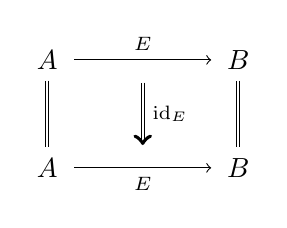
\begin{tikzpicture}[x=1.5em,y=1.5em]
  \node (At) at (0,1.3)    {$A$};
  \node (Bt) at (4.6,1.3)  {$B$};
  \node (Ab) at (0,-1.3)   {$A$};
  \node (Bb) at (4.6,-1.3) {$B$};
  \draw[->] (0.65,1.3) -- node[above]{$\scriptstyle E$} (3.95,1.3);
  \draw[->] (0.65,-1.3) -- node[below]{$\scriptstyle E$} (3.95,-1.3);
  \draw[double] (0,0.8) -- (0,-0.8);
  \draw[double] (4.6,0.8) -- (4.6,-0.8);
  \draw[double,->] (2.3,0.75) -- node[right]{$\scriptstyle\mathrm{id}_{E}$} (2.3,-0.75);
\end{tikzpicture}
\end{center}
\end{itemize}
使得胞腔的复合在通常的多范畴意义下既是结合的又是幺的。
\end{definition}

\begin{lemma}\label{lem:virtual-double-category-of-two-sided-isofibrations}
存在一个双侧等价纤维化的\trVirtualDoubleCategory{}，其中：
\begin{itemize}
\item \textbf{对象}为\trInfinityCategories{}；
\item \textbf{竖直箭头}为\trFunctor{}；
\item \textbf{水平箭头}为双侧等价纤维化；并且
\item $n$ 元\textbf{\trCell}（\eqref{eq:virtual-cell-boundary}）是位于
$f\times g$ 之上的双侧等价纤维化之间的映射
\begin{rveq}\label{eq:n-ary-cell-as-map}
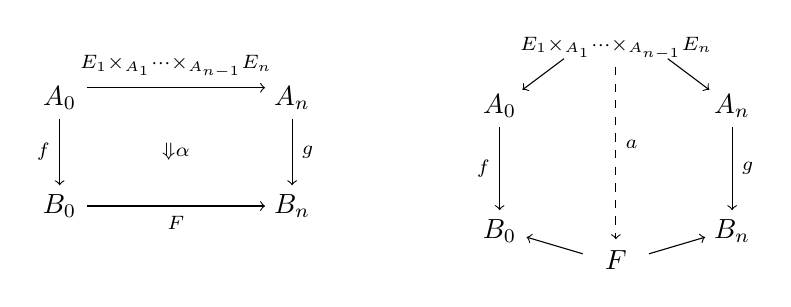
\begin{tikzpicture}[x=1.5em,y=1.5em]
  \node (A0) at (0,1.3)    {$A_{0}$};
  \node (An) at (5.6,1.3)  {$A_{n}$};
  \draw[->] (0.65,1.55) --
    node[above]{$\scriptstyle E_{1}\times_{A_{1}}\cdots\times_{A_{n-1}}E_{n}$} (4.95,1.55);
  \node (B0) at (0,-1.3)   {$B_{0}$};
  \node (Bn) at (5.6,-1.3) {$B_{n}$};
  \draw[->] (0,0.8) -- node[left]{$\scriptstyle f$} (0,-0.8);
  \draw[->] (5.6,0.8) -- node[right]{$\scriptstyle g$} (5.6,-0.8);
  \node at (2.8,0) {$\scriptstyle\Downarrow\alpha$};
  \draw[->] (0.65,-1.3) -- node[below]{$\scriptstyle F$} (4.95,-1.3);
  \node at (7.9,0) {$\leftrightsquigarrow$};
  \begin{scope}[shift={(10.6,0)}]
  \node (P) at (2.8,2.5)
    {$\scriptstyle E_{1}\times_{A_{1}}\cdots\times_{A_{n-1}}E_{n}$};
  \node (a0) at (0,1.1)   {$A_{0}$};
  \node (an) at (5.6,1.1) {$A_{n}$};
  \draw[->] (1.55,2.25) -- (0.55,1.5);
  \draw[->] (4.05,2.25) -- (5.05,1.5);
  \draw[->,dashed] (2.8,2.05) -- node[right,pos=0.45]{$\scriptstyle a$} (2.8,-2.1);
  \node (b0) at (0,-1.9)   {$B_{0}$};
  \node (bn) at (5.6,-1.9) {$B_{n}$};
  \draw[->] (0,0.6) -- node[left]{$\scriptstyle f$} (0,-1.4);
  \draw[->] (5.6,0.6) -- node[right]{$\scriptstyle g$} (5.6,-1.4);
  \node (F) at (2.8,-2.6) {$F$};
  \draw[->] (2.0,-2.45) -- (0.65,-2.05);
  \draw[->] (3.6,-2.45) -- (4.95,-2.05);
  \end{scope}
\end{tikzpicture}
\end{rveq}
其唯一的竖直源是 \eqref{eq:virtual-cell-boundary} 中构成其水平源\footnote{%
原书两处均印作「vertical」：此处作「comprising the vertical source in
(8.1.9)」（构成 (8.1.9) 中竖直源的……），零元段作「which have an empty
sequence as their vertical domain」（以空序列为其竖直定义域）。按定义
8.1.8，(8.1.9) 中那列跨度构成胞腔的水平源、空序列构成零元胞腔的水平%
定义域（对照原书 p.313 平行句「comprising the horizontal source in the
left-hand diagram」即作 horizontal），疑两处「vertical」均为
「horizontal」之排印误，此处一并径改。——译者注}的那列跨度的 $(n-1)$ 重跨度复合。
\end{itemize}
\end{lemma}

\begin{proof}
所需的诸复合定律可以这样定义：把诸\trVirtualDoubleCategory{}嵌入到%
\cref{prop:double-category-of-two-sided-isofibrations}的诸\trDoubleCategory{}之中。
例如，\eqref{eq:virtual-composite-cell} 左侧所示的那个构型，其复合可以
定义为：先在等价纤维化的\trDoubleCategory{}中把顶部的 $k$ 支胞腔作水平复合，再把结果
与底部的胞腔作竖直复合。其结果即\trVirtualDoubleCategory{}中一支形状正确的
$k_{1}+\cdots+k_{n}$ 元胞腔。

尚待定义的只是零元胞腔\footnote{注意记号 $\rvnullpair$ 之使用：它表示
一支零元胞腔的零元源；采用这一记号，是为了让此类胞腔得以自然地纳入虚拟%
\trDoubleCategory{}中诸胞腔的\trPastingDiagram{}。}
——即以空序列为其水平定义域的那些胞腔
\begin{center}
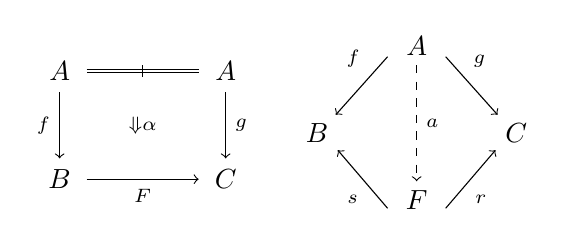
\begin{tikzpicture}[x=1.5em,y=1.5em]
  \node (At) at (0,1.3)   {$A$};
  \node (At2) at (4.0,1.3){$A$};
  \node (B)  at (0,-1.3)  {$B$};
  \node (C)  at (4.0,-1.3){$C$};
  \draw[double] (0.65,1.3) -- (3.35,1.3);
  \draw (2.0,1.45) -- (2.0,1.15);
  \draw[->] (0.65,-1.3) -- node[below]{$\scriptstyle F$} (3.35,-1.3);
  \draw[->] (0,0.8) -- node[left]{$\scriptstyle f$} (0,-0.8);
  \draw[->] (4.0,0.8) -- node[right]{$\scriptstyle g$} (4.0,-0.8);
  \node at (2.0,0) {$\scriptstyle\Downarrow\alpha$};
  \node at (6.3,0) {$\leftrightsquigarrow$};
  \begin{scope}[shift={(8.6,0)}]
  \node (nA) at (0,1.9)    {$A$};
  \node (nB) at (-2.4,-0.2){$B$};
  \node (nC) at (2.4,-0.2) {$C$};
  \draw[->] (-0.7,1.65) -- node[above left,pos=0.35]{$\scriptstyle f$} (-1.95,0.25);
  \draw[->] (0.7,1.65)  -- node[above right,pos=0.35]{$\scriptstyle g$} (1.95,0.25);
  \draw[->,dashed] (0,1.45) -- node[right,pos=0.5]{$\scriptstyle a$} (0,-1.35);
  \node (nF) at (0,-1.8) {$F$};
  \draw[->] (-0.7,-2.0) -- node[below left,pos=0.4]{$\scriptstyle s$} (-1.9,-0.6);
  \draw[->] (0.7,-2.0)  -- node[below right,pos=0.4]{$\scriptstyle r$} (1.9,-0.6);
  \end{scope}
\end{tikzpicture}
\end{center}
我们把它解读为一个 0 重拉回，这即是从 $A$ 到 $A$ 的恒同跨度。于是，上方
左图所展示的零元胞腔是上方右图所示诸映射的纤维化同构类，其中 $a$ 与 $a'$
位于同一个等价类中，当存在自然同构 $\gamma\colon a\cong a'$ 使得
$s\gamma=\mathrm{id}_{f}$ 且 $r\gamma=\mathrm{id}_{g}$。
\end{proof}

\begin{remark}\label{rem:diagonal-nullary-morphism}
例如，映射
\begin{center}
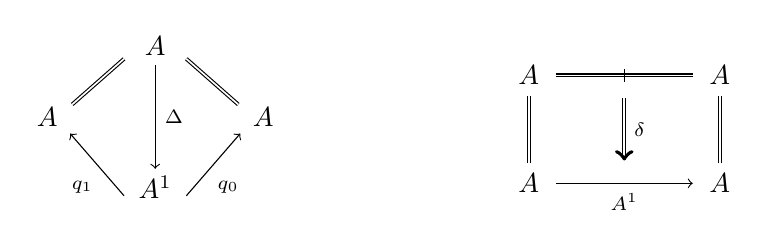
\begin{tikzpicture}[x=1.5em,y=1.5em]
  \begin{scope}[shift={(0,0)}]
  \node (At) at (0,2.0)    {$A$};
  \node (Al) at (-2.6,0.3) {$A$};
  \node (Ar) at (2.6,0.3)  {$A$};
  \node (Ab) at (0,-1.4)   {$A^{\mathbb{1}}$};
  \draw[double] (-0.75,1.7) -- (-2.0,0.6);
  \draw[double] (0.75,1.7)  -- (2.0,0.6);
  \draw[->] (0,1.55) -- node[right,pos=0.5]{$\scriptstyle\Delta$} (0,-0.95);
  \draw[->] (-0.75,-1.6) -- node[below left,pos=0.4]{$\scriptstyle q_{1}$} (-2.05,-0.1);
  \draw[->] (0.75,-1.6)  -- node[below right,pos=0.4]{$\scriptstyle q_{0}$} (2.05,-0.1);
  \end{scope}
  \node at (5.4,0.2) {$\leftrightsquigarrow$};
  \begin{scope}[shift={(9.0,0)}]
  \node (a) at (0,1.3)    {$A$};
  \node (b) at (4.6,1.3)  {$A$};
  \node (c) at (0,-1.3)   {$A$};
  \node (d) at (4.6,-1.3) {$A$};
  \draw[double] (0.65,1.3) -- (3.95,1.3);
  \draw (2.3,1.45) -- (2.3,1.15);
  \draw[->] (0.65,-1.3) -- node[below]{$\scriptstyle A^{\mathbb{1}}$} (3.95,-1.3);
  \draw[double] (0,0.8) -- (0,-0.8);
  \draw[double] (4.6,0.8) -- (4.6,-0.8);
  \draw[double,->] (2.3,0.75) -- node[right]{$\scriptstyle\delta$} (2.3,-0.75);
  \end{scope}
\end{tikzpicture}
\end{center}
在双侧等价纤维化的\trVirtualDoubleCategory{}中定义了一个余定义域为
$A\xrightarrow{A^{\mathbb{1}}}A$ 的零元态射。然而请注意：尽管
$\Delta\colon A\simeq A^{\mathbb{1}}$ 在周围的∞-宇宙中定义了一个%
\trEquivalence{}，这个胞腔在任何一种\trVirtualDoubleCategory{}中都不定义\trIsomorphism{}。
这一零元态射赋予 $A\xrightarrow{A^{\mathbb{1}}}A$ 一种适合\trVirtualDoubleCategory{}的
单位结构（见练习 8.2.iii）。正是因为这类原因，我们在%
\cref{prop:double-category-of-two-sided-isofibrations}中略去了水平的恒同
箭头。
\end{remark}

我们感兴趣的主要例子，是一个通过限制水平箭头的类、并取其之间的全部胞腔
而定义的全子\trVirtualDoubleCategory{}。
由于\trVirtualDoubleCategory{}的结构中给出的运算仅有竖直源与竖直靶、竖直恒同以及竖直
复合，显然这一子结构在这些运算之下全部封闭，从而继承\trVirtualDoubleCategory{}的结构。

\begin{corollary}\label{cor:virtual-double-category-of-modules}
对任意∞-宇宙 $\mathcal{K}$，存在一个\trModule{}的\trVirtualDoubleCategory
$\Mod(\mathcal{K})$，它定义为等价纤维化的\trVirtualDoubleCategory{}的一个全子范畴，其中：
\begin{itemize}
\item \textbf{对象}为\trInfinityCategories{}；
\item \textbf{竖直箭头}为\trFunctor{}；
\item \textbf{水平箭头} $A\xrightarrow{E}B$ 是从 $A$ 到 $B$ 的\trModule{}
$E$；
\item $n$ 元\textbf{\trCell}是位于 $f\times g$ 之上的、双侧等价纤维化之间
的映射的纤维化同构类：
\begin{rveq}\label{eq:n-ary-module-map}
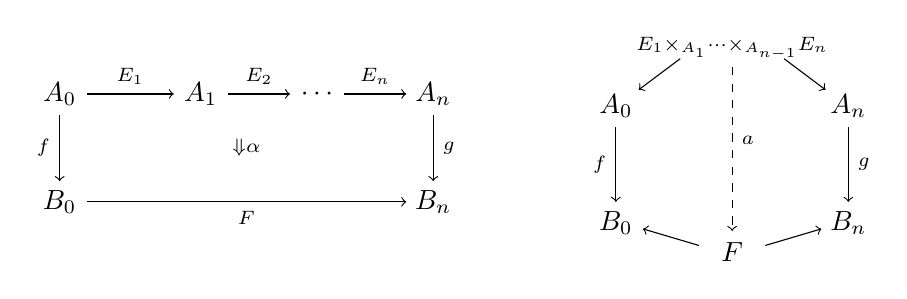
\begin{tikzpicture}[x=1.5em,y=1.5em]
  \node (A0) at (0,1.3)    {$A_{0}$};
  \node (A1) at (3.4,1.3)  {$A_{1}$};
  \node (Ad) at (6.2,1.3)  {$\cdots$};
  \node (An) at (9.0,1.3)  {$A_{n}$};
  \draw[->] (0.65,1.3) -- node[above]{$\scriptstyle E_{1}$} (2.75,1.3);
  \draw[->] (4.05,1.3) -- node[above]{$\scriptstyle E_{2}$} (5.55,1.3);
  \draw[->] (6.85,1.3) -- node[above]{$\scriptstyle E_{n}$} (8.35,1.3);
  \node (B0) at (0,-1.3)   {$B_{0}$};
  \node (Bn) at (9.0,-1.3) {$B_{n}$};
  \draw[->] (0,0.8) -- node[left]{$\scriptstyle f$} (0,-0.8);
  \draw[->] (9.0,0.8) -- node[right]{$\scriptstyle g$} (9.0,-0.8);
  \node at (4.5,0) {$\scriptstyle\Downarrow\alpha$};
  \draw[->] (0.65,-1.3) -- node[below]{$\scriptstyle F$} (8.35,-1.3);
  \node at (11.3,0) {$\leftrightsquigarrow$};
  \begin{scope}[shift={(13.4,0)}]
  \node (P) at (2.8,2.4)
    {$\scriptstyle E_{1}\times_{A_{1}}\cdots\times_{A_{n-1}}E_{n}$};
  \node (a0) at (0,1.0)   {$A_{0}$};
  \node (an) at (5.6,1.0) {$A_{n}$};
  \draw[->] (1.55,2.15) -- (0.55,1.4);
  \draw[->] (4.05,2.15) -- (5.05,1.4);
  \draw[->,dashed] (2.8,1.95) -- node[right,pos=0.45]{$\scriptstyle a$} (2.8,-2.0);
  \node (b0) at (0,-1.8)   {$B_{0}$};
  \node (bn) at (5.6,-1.8) {$B_{n}$};
  \draw[->] (0,0.5) -- node[left]{$\scriptstyle f$} (0,-1.3);
  \draw[->] (5.6,0.5) -- node[right]{$\scriptstyle g$} (5.6,-1.3);
  \node (F) at (2.8,-2.5) {$F$};
  \draw[->] (2.0,-2.35) -- (0.65,-1.95);
  \draw[->] (3.6,-2.35) -- (4.95,-1.95);
  \end{scope}
\end{tikzpicture}
\end{rveq}
\end{itemize}
\end{corollary}

\eqref{eq:n-ary-module-map} 的\textbf{$n$ 元模映射}（n-ary module maps）
可以设想为\cref{lem:virtual-double-category-of-two-sided-isofibrations}
的 $n$ 元胞腔的特例，其中 $E_{1},\ldots,E_{n}$ 与 $F$ 全都被要求是%
\trModule{}：图表 \eqref{eq:n-ary-cell-as-map} 中那个唯一的水平源，是由左图
中构成水平源的那列\trModule{}经 $n-1$ 重\trPullback{}所定义的那条%
\trTwoSidedFibration{}。
我们把作为一支 $n$ 元模映射的水平定义域出现的那列有限的\trModule{}称为
一个\textbf{模的相容序列}（compatible sequence of modules）；这只意味着：
它们的水平源与水平靶以显见的方式相容。

下面这个特殊情形，给出了这种 $n$ 元模映射概念何以切题的一个暗示。

\begin{lemma}\label{lem:comma-module-maps-bijection}
在如下两类东西之间存在一个双射：其一，余定义域\trModule{}为下左图所示的
逗号\trModule{}的那些 $n$ 元模映射；其二，\trHomotopyTwoCategory{}中边界
为下右图所示的那些\trNaturalTransformation{}：
\begin{center}
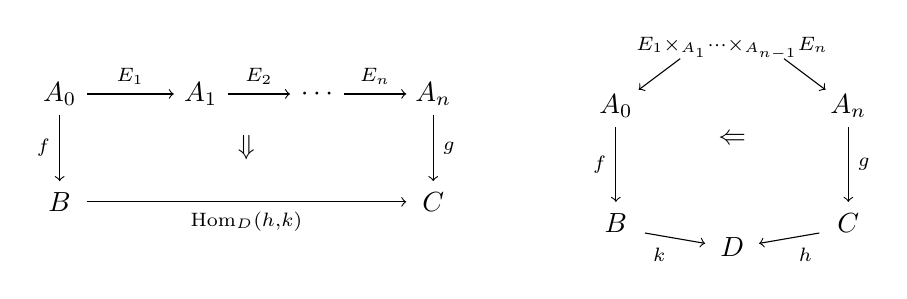
\begin{tikzpicture}[x=1.5em,y=1.5em]
  \node (A0) at (0,1.3)    {$A_{0}$};
  \node (A1) at (3.4,1.3)  {$A_{1}$};
  \node (Ad) at (6.2,1.3)  {$\cdots$};
  \node (An) at (9.0,1.3)  {$A_{n}$};
  \draw[->] (0.65,1.3) -- node[above]{$\scriptstyle E_{1}$} (2.75,1.3);
  \draw[->] (4.05,1.3) -- node[above]{$\scriptstyle E_{2}$} (5.55,1.3);
  \draw[->] (6.85,1.3) -- node[above]{$\scriptstyle E_{n}$} (8.35,1.3);
  \node (B) at (0,-1.3) {$B$};
  \node (C) at (9.0,-1.3){$C$};
  \draw[->] (0,0.8) -- node[left]{$\scriptstyle f$} (0,-0.8);
  \draw[->] (9.0,0.8) -- node[right]{$\scriptstyle g$} (9.0,-0.8);
  \node at (4.5,0) {$\Downarrow$};
  \draw[->] (0.65,-1.3) -- node[below]{$\scriptstyle\mathrm{Hom}_{D}(h,k)$} (8.35,-1.3);
  \node at (11.3,0) {$\leftrightsquigarrow$};
  \begin{scope}[shift={(13.4,0)}]
  \node (P) at (2.8,2.4)
    {$\scriptstyle E_{1}\times_{A_{1}}\cdots\times_{A_{n-1}}E_{n}$};
  \node (a0) at (0,1.0)   {$A_{0}$};
  \node (an) at (5.6,1.0) {$A_{n}$};
  \draw[->] (1.55,2.15) -- (0.55,1.4);
  \draw[->] (4.05,2.15) -- (5.05,1.4);
  \node at (2.8,0.2) {$\Leftarrow$};
  \node (b) at (0,-1.8)  {$B$};
  \node (d) at (2.8,-2.4){$D$};
  \node (c) at (5.6,-1.8){$C$};
  \draw[->] (0,0.5) -- node[left]{$\scriptstyle f$} (0,-1.3);
  \draw[->] (5.6,0.5) -- node[right]{$\scriptstyle g$} (5.6,-1.3);
  \draw[->] (0.7,-2.05) -- node[below left,pos=0.5]{$\scriptstyle k$} (2.15,-2.3);
  \draw[->] (4.9,-2.05) -- node[below right,pos=0.5]{$\scriptstyle h$} (3.45,-2.3);
  \end{scope}
\end{tikzpicture}
\end{center}
\end{lemma}

\begin{proof}
把\cref{def:maps-in-squares}与命题 3.4.7 结合起来。
\end{proof}

对于模的\trVirtualDoubleCategory{}中的任意一对对象 $A$ 与 $B$，存在一个竖直 1-范畴，其
对象为从 $A$ 到 $B$ 的\trModule{}、其态射为位于一对恒同\trFunctor{}之上的
模映射；这个范畴与\cref{obs:one-categories-of-modules}中引入的从 $A$ 到
$B$ 的模的 1-范畴相重合。在这一语境下，%
\cref{lem:one-category-equivalences}可以重述如下：

\begin{lemma}\label{lem:module-vertical-isomorphism}
一对平行的\trModule{} $A\xrightarrow{E}B$ 与 $A\xrightarrow{F}B$ 作为模的%
\trVirtualDoubleCategory{}中模的竖直 1-范畴的对象而同构，当且仅当
$E\simeq_{A\times B}F$。
\end{lemma}

为了与全书其余部分保持一致，凡当\trModule{} $A\xrightarrow{E}B$ 与
$A\xrightarrow{F}B$ 作为从 $A$ 到 $B$ 的模的竖直 1-范畴中的对象同构时，
我们就写作 $E\simeq F$ 或 $E\simeq_{A\times B}F$。例如，命题 4.1.1 证明：
一个\trFunctor{} $f\colon B\to A$ 作为一个\trFunctor{} $u\colon A\to B$
的\trLeftAdjoint{}，当且仅当
$\mathrm{Hom}_{A}(f,A)\simeq_{A\times B}\mathrm{Hom}_{B}(B,u)$；也就是说，
当且仅当诸\trModule{} $A\xrightarrow{\mathrm{Hom}_{A}(f,A)}B$\footnote{%
原书印作「$B\xrightarrow{\mathrm{Hom}_{A}(f,A)}A$」。按本书模的方向约定
（第 7 章定义 7.4.7：$\mathrm{Hom}_{B}(B,f)$ 是从 $A$ 到 $B$ 的模），%
$\mathrm{Hom}_{A}(f,A)$ 应为从 $A$ 到 $B$ 的模，且与本句末「从 $A$ 到
$B$ 的模的竖直 1-范畴」相合；第一支模疑为
「$A\xrightarrow{\mathrm{Hom}_{A}(f,A)}B$」之误，此处径改。——译者注}
与 $A\xrightarrow{\mathrm{Hom}_{B}(B,u)}B$ 作为从 $A$ 到 $B$ 的模的竖直
1-范畴中的对象同构。

\subsection*{练习}

\begin{exercise}\label{ex:cosmos-of-two-sided-isofibrations}
由练习 6.1.iii，对任意∞-宇宙 $\mathcal{K}$，存在一个∞-宇宙
$\mathcal{K}^{\times}$，其对象为任意一对∞-范畴之间的双侧等价纤维化——
这些恰好是由该\trSpan{}所标引的「\trFibrant{}图表」，其中该\trSpan{}被
视为一个逆范畴。
请把这个∞-宇宙连同诸端点求值\trFunctor{}
$\mathcal{K}^{\times}\to\mathcal{K}$ 一起使用，给出双侧等价纤维化的\trDoubleCategory
的第二个描述——把它描述为在∞-宇宙、\trCosmologicalFunctor{}与%
\trSimplicial{}自然同构的层面上定义的一个非幺内范畴的商。\footnote{我们
认为下述问题是一个未决问题：在双侧等价纤维化的非幺\trDoubleCategory{}或模的虚拟双
范畴上安置一个「双重拟范畴」是否有用。}
\end{exercise}

\begin{exercise}\label{ex:double-defines-virtual}
证明：任何\trDoubleCategory{}都定义一个\trVirtualDoubleCategory{}。\footnote{若该\trDoubleCategory{}缺乏水平的恒同
态射，则相应的\trVirtualDoubleCategory{}可能缺乏零元态射——除非这些态射能够以某种别的
方式定义，正如我们在\cref{lem:virtual-double-category-of-two-sided-isofibrations}
的证明中所做的那样。}
\end{exercise}

\begin{exercise}\label{ex:three-bijections-from-yoneda}
用定理 7.4.8 的三条陈述，描述模的\trVirtualDoubleCategory{}中具有各种边界形状的胞腔之间
的三个双射。
\end{exercise}

\begin{exercise}\label{ex:map-of-two-sided-fibrations}
设 $A\overset{q}{\twoheadleftarrow}E\overset{p}{\twoheadrightarrow}B$ 与
$A\overset{s}{\twoheadleftarrow}F\overset{r}{\twoheadrightarrow}B$ 是两条%
\trTwoSidedFibration{}。从
$A\overset{q}{\twoheadleftarrow}E\overset{p}{\twoheadrightarrow}B$ 到
$A\overset{s}{\twoheadleftarrow}F\overset{r}{\twoheadrightarrow}B$ 的一支%
\textbf{双侧纤维化映射}（map of two-sided fibrations），是一个由严格交换
的\trFunctor{} $a$ 构成的纤维化同构类，使得左方形在诸%
\trCocartesianFibration{}之间定义一个\trCartesianFunctor{}，而右方形在诸%
\trCartesianFibration{}之间定义一个\trCartesianFunctor{}（见命题 7.1.7）。
\begin{center}
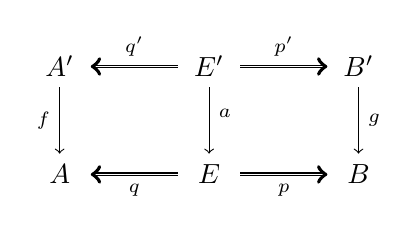
\begin{tikzpicture}[x=1.5em,y=1.5em]
  \node (Ap) at (0,1.3)    {$A'$};
  \node (Ep) at (3.6,1.3)  {$E'$};
  \node (Bp) at (7.2,1.3)  {$B'$};
  \node (A)  at (0,-1.3)   {$A$};
  \node (E)  at (3.6,-1.3) {$E$};
  \node (B)  at (7.2,-1.3) {$B$};
  \draw[double,->] (2.85,1.3) -- node[above]{$\scriptstyle q'$} (0.75,1.3);
  \draw[double,->] (4.35,1.3) -- node[above]{$\scriptstyle p'$} (6.45,1.3);
  \draw[double,->] (2.85,-1.3) -- node[below]{$\scriptstyle q$} (0.75,-1.3);
  \draw[double,->] (4.35,-1.3) -- node[below]{$\scriptstyle p$} (6.45,-1.3);
  \draw[->] (0,0.8) -- node[left]{$\scriptstyle f$} (0,-0.8);
  \draw[->] (3.6,0.8) -- node[right,pos=0.4]{$\scriptstyle a$} (3.6,-0.8);
  \draw[->] (7.2,0.8) -- node[right]{$\scriptstyle g$} (7.2,-0.8);
\end{tikzpicture}
\end{center}
请定义一个双侧纤维化的\trDoubleCategory{}：作为\cref{prop:double-category-of-two-sided-isofibrations}
的双侧等价纤维化\trDoubleCategory{}的一个非全子范畴。
\end{exercise}

